\chapter{Σχεδίαση \& Υλοποίηση}
Σε αυτό το κεφάλαιο γίνεται ανάλυση του συστήματος στα επιμέρους μέρη και περιγράφεται η διαδικασία της υλοποίησης τους. Επεξηγούνται επίσης τα σημαντικότερα σημεία στον κώδικα και οι αλγόριθμοι που χρησιμοποιούνται για την επίλυση των κυριότερων λειτουργιών. Έχουν συμπεριληφθεί τμήματα κώδικα αλλά και διαγράμματα τα οποία βοηθούν στην κατανόηση των λύσεων που έχουν χρησιμοποιηθεί.

%% ================================================== 
%% ΔΕΔΟΜΕΝΑ ΣΥΣΤΗΜΑΤΟΣ
%% ==================================================
\section{Δεδομένα Συστήματος}
Το κυριότερο πρόβλημα που προσπαθεί να λύσει το σύστημα είναι η κράτηση και η διαχείριση ραντεβού από μια επιχείριση. Σε αυτήν την περίπτωση χρήσης έχει επικεντρωθεί η σχεδίαση και η υλοποίηση του συστήματος το οποίο περιέχει και άλλες δυνατότητες οι οποίες μπορούν όμως να θεωρηθούν λιγότερο σημαντικές. Έχοντας υπόψιν την έννοια "ραντεβού" ως την κύρια οντότητα της εφαρμογής, σχεδιάστηκε το παρακάτω μοντέλο το οποίο διευκρινίζει τις σχέσεις των υπόλοιπων οντοτήτων σε σχέση με το ραντεβού αλλά και μεταξύ τους.

\begin{figure}[ht!]
\centering
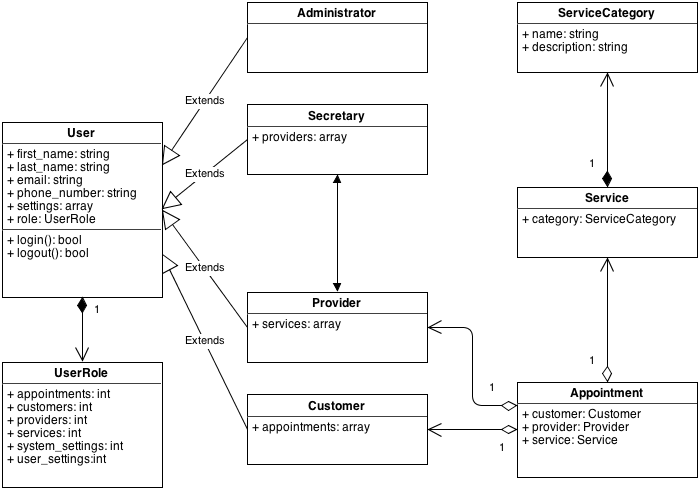
\includegraphics[width=160mm]{images/domain-model.png}
\caption{Domain model του συστήματος}
\label{domain-model}
\end{figure}

Με βάση αυτό το σχεδιάγραμμα μπορεί πολύ εύκολα να προκύψει και το σχεδιακό μοντέλο της βάσης δεδομένων, δεδομένου ότι έχουμε και τις οντότητες, αλλά και τις σχέσεις μεταξύ τους. Όλοι οι χρήστες της εφαρμογής κληρονομούν την συμπεριφορά τους από μια οντότητα (User) και στην συνέχεια προσθέτουν τις πρόσθετες ιδιαιτερότητες που τους χαρακτηρίζουν. Για παράδειγμα ο χρήστης γραμματέας (Secretary) περιέχει έναν πίνακα από πάροχους (Providers) τους οποίους μπορεί να διαχειριστεί, ή ένα ραντεβού είναι ξεκάθαρο ότι περιέχει στην πληροφορία του έναν πελάτη, έναν πάροχο και μια υπηρεσία.

\begin{figure}[ht!]
\centering
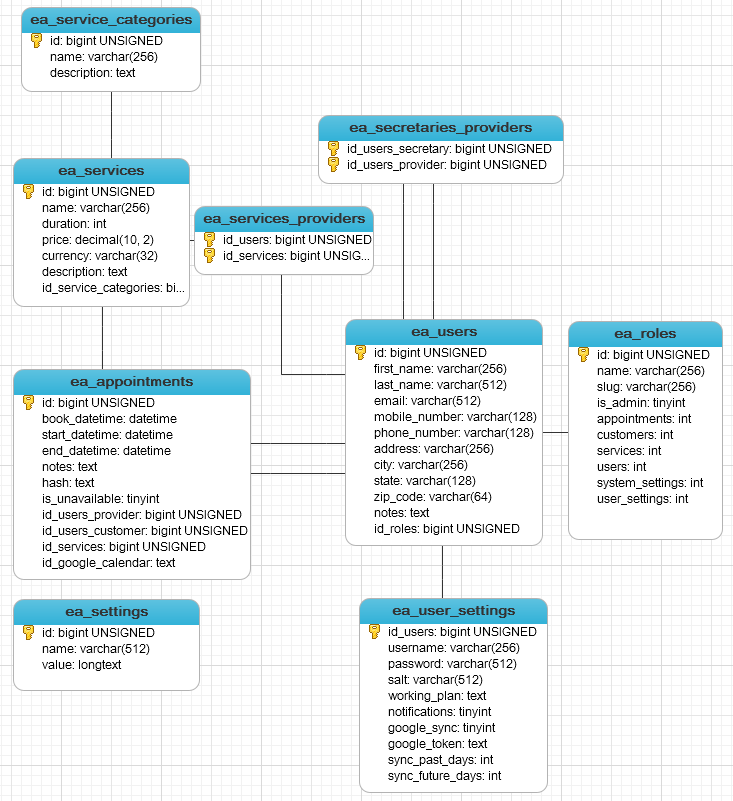
\includegraphics[width=160mm]{images/er.png}
\caption{Σχεσιακό μοντέλο της βάσης δεδομένων (ER).}
\label{er}
\end{figure}

Για την διαχείριση των δεδομένων της βάσης δημιουργήθηκαν ειδικές κλάσεις (models) οι οποίες περιέχουν μεθόδους που χρησιμοποιούνται από τους controllers του συστήματος. Το CodeIgniter δίνει στον προγραμματιστή ένα δικό του μέσο επικοινωνίας με την βάση δεδομένων, το οποίο είναι ένα πολύ ισχυρό και ευέλικτο εργαλείο. Η επονομαζόμενη Database Class του CodeIgniter επιτρέπει στον προγραμματιστεί να εκτελεί ερωτήματα προς την βάση, να παράγει αποτελέσματα και να τα αναλύει σε ξεχωριστές εγγραφές, να κρατάει στην μνήμη ερωτήματα για γρηγορότερη ανταπόκριση (query caching) και κυριότερο την κλάση Active Record. Η κλάση αυτή έχει έναν δικό της τρόπο για την εκτέλεση των ερωτημάτων προς την βάση. Όλα τα τμήματα ενός τυπικού ερωτήματος είναι μέθοδοι σε αυτήν την κλάση και έτσι ο προγραμματιστείς χρησιμοποιεί τις μεθόδους αυτές για να επικοινωνήσει με την βάση δεδομένων. Το θετικό είναι ότι ανεξαρτήτως τον τύπο της βάσης η κλάση αυτή λειτουργεί με τον ίδιο τρόπο (MySQL, PostGre, MSSQL κτλ). Η τεχνική αυτή λέγεται Active Record Database Pattern και έχει αν κάνει με την αλλαγή adapter στην κλάση ανάλογα με τον τύπο της βάσης. Σε κάθε περίπτωση όμως ο τρόπος λειτουργίας της είναι ο ίδιος. Στο παρακάτω τμήμα κώδικα αναφέρεται ένα παράδειγμα για το πως μπορεί να βρεθεί το αναγνωριστικό μιας εγγραφής χρησιμοποιώντας ως κλειδί την διεύθυνση email.

\begin{verbatim}
public function find_record_id($admin) {
  if (!isset($admin['email'])) {
    throw new Exception('Admin email was not provided: ' 
	    . print_r($admin, TRUE));
  }
	
  $result = $this->db
      ->select('ea_users.id')
      ->from('ea_users')
      ->join('ea_roles', 'ea_roles.id = ea_users.id_roles', 'inner')
      ->where('ea_users.email', $admin['email'])
      ->where('ea_roles.slug', DB_SLUG_ADMIN)
      ->get();
	
  if ($result->num_rows() == 0) {
    throw new Exception('Could not find admin record id.');
  }
	
  return intval($result->row()->id);
}
\end{verbatim}

%% ================================================== 
%% ΑΡΧΙΤΕΚΤΟΝΙΚΗ ΤΟΥ ΚΩΔΙΚΑ
%% ==================================================
\section{Αρχιτεκτονική Του Κώδικα}
Η εφαρμογή είναι γραμμένη χρησιμοποιώντας τις εξής τεχνολογίες: PHP, Javascript, HTML, CSS, MySQL. Εκτός αυτών έχουν χρησιμοποιηθεί και κάποια βοηθητικά εργαλεία τα οποία διευκολύνουν τον προγραμματιστή στο να πετύχει καλύτερο αποτέλεσμα σε μικρότερο χρόνο. Αυτά τα εργαλεία (frameworks) όπως έχουν αναφερθεί και σε προηγούμενο κεφάλαιο είναι τα CodeIgniter (PHP), jQuery (Javascript), Bootstrap (CSS + Javascript). 

Όσον αφορά την αρχιτεκτονική του κώδικα έχει επιλεχθεί το μοντέλο MVC (Model - View - Controller) και αυτό υλοποιείται με την χρήση του CodeIgniter με άριστη απόδοση. Ο κώδικας PHP έχει χωριστεί σε τρία μέρη και έτσι χρησιμοποιείται σε όλη την εφαρμογή. Με αυτόν τον τρόπο βελτιώνονται οι συνθήκες συντήρησης γιατί είναι ξεκάθαρο σε ποιο από τα τρία ξεχωριστά σημεία ανήκει ένα τμήμα κώδικα. Έχουν συγγραφεί και δοκιμαστεί κλάσεις models για κάθε οντότητα οι οποίες αναλαμβάνουν την διαχείριση των δεδομένων με την βάση. Επίσης έχουν δημιουργηθεί views για κάθε σελίδα που πιθανόν θα δει ο χρήστης τα οποία συνδέονται με ένα κομμάτι CSS κώδικα, υπεύθυνο για την μορφοποίηση της σελίδας. Τέλος τον συντονισμό των προηγούμενων αναλαμβάνουν οι κλάσεις controllers οι οποίες είτε είναι υπεύθυνες για την  σωστή φόρτωση μιας σελίδας της εφαρμογής είτε απαντούν σε κλήσεις της JavaScript που γίνονται μέσω της τεχνολογίας AJAX.

Πολύ μεγάλο μέρος της εφαρμογής έχει γραφτεί σε JavaScript για να μπορέσει το περιβάλλον εργασίας του χρήστη να γίνει αρκετά φιλικό και οικείο. Το κομμάτι JavaScript κώδικα χωρίζεται σε διάφορες κλάσεις και namespace τα οποία χρησιμοποιούνται από μια ή και παραπάνω σελίδες και στόχο έχουν να "ζωντανέψουν" το περιεχόμενο προσθέτοντας διαδραστικότητα. Πολλές φορές είναι απαραίτητο να εκτελεστούν κλήσεις AJAX προς τον server για την λήψη πρόσθετων πληροφοριών, είτε για να αποσταλούν δεδομένα τα οποία σηματοδοτούν για παράδειγμα κάποια επεξεργασία ή και διαγραφή εγγραφής από την βάση δεδομένων. Το framework jQuery αποτελεί σημαντικό εργαλείο για την διεκπεραίωση αυτής της λειτουργίας διότι δίνει την δυνατότητα στον προγραμματιστή να γράψει κώδικα όμορφα δομημένο και πολύ αποδοτικό, από ότι θα ήταν χωρίς την χρήση του. Αυτή η ιδιότητα της βιβλιοθήκης συντελεί και στην δημοτικότητά της και την χρήση της από κολοσσούς ανάπτυξης λογισμικού.

Για την μορφοποίηση των σελίδων της εφαρμογής χρησιμοποιήθηκε το πιο διαδεδομένο CSS framework αυτήν την περίοδο, το Bootstap. Χρησιμοποιώντας αυτό το framework γράφτηκε νέο CSS το οποίο μορφοποιεί τις σελίδες έτσι ώστε να ανταποκρίνονται όπως πρέπει σε διάφορα μεγέθη οθονών.

Στο παρακάτω σχεδιάγραμμα γίνεται σαφής ο διαχωρισμός του κώδικα του συστήματος στα διάφορα τμήματα που το απαρτίζουν και η χρήση των εξωτερικών εργαλείων που συντέλεσαν στην ορθή ανάπτυξη της εφαρμογής.

\begin{figure}[ht!]
\centering
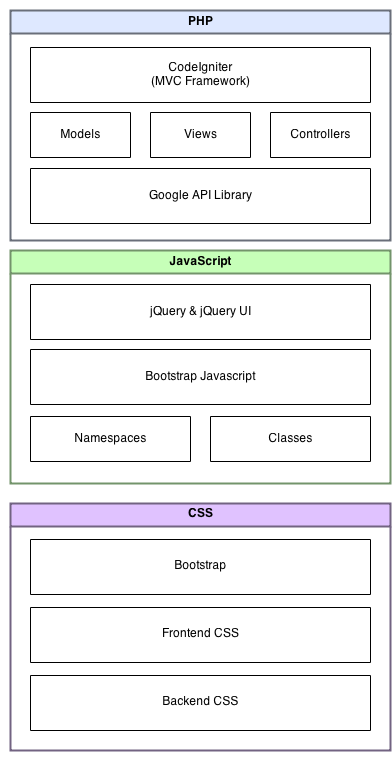
\includegraphics[width=100mm]{images/system-architecture.png}
\caption{Τα τμήματα που απαρτίζουν το Easy!Appointments.}
\label{system-architecture}
\end{figure}

%% ================================================== 
%% ΥΛΟΠΟΙΗΣΗ ΤΟΥ ΣΥΣΤΗΜΑΤΟΣ
%% ==================================================
\section{Υλοποίηση Του Συστήματος}
Εφόσον ο αρχικός σχεδιασμός είχε ολοκληρωθεί ξεκίνησε η υλοποίηση της εφαρμογής με πρώτη εργασία τον σχεδιασμό της βάσης δεδομένων. Έχοντας ήδη σχεδιασμένο το domain model η δημιουργία του σχήματος της βάσης έγινε γρήγορα και διατηρήθηκε ως την ολοκλήρωση του έργου με μικρές προσθήκες όπου ήταν απαραίτητο. 

Στην συνέχεια, πριν γραφεί κώδικας θα έπρεπε να γίνει η επιλογή και το στήσιμο των εξωτερικών βιβλιοθηκών που θα κρίνονταν απαραίτητα για την λειτουργία του συστήματος. Σε αυτήν την φάση επιλέχθηκαν οι βασικές βιβλιοθήκες (CodeIgniter, Google API Library, jQuery, Bootstrap) και επιλέχθηκε η σημαντικότερη περίπτωση χρήσης για να υλοποιηθεί πρώτη. Αυτή δεν ήταν άλλη από την κράτηση ενός ραντεβού από τον πελάτη. Επιλέχθηκε αυτή η περίπτωση χρήσης γιατί με αυτόν τον τρόπο θα καθορίζονταν εν μέρη και η αρχιτεκτονική του συστήματος καθώς αυτό θα εξελισσόταν σταδιακά με την ολοκλήρωση και των υπόλοιπων περιπτώσεων χρήσης.

Η κύρια ροή εργασιών ως προς την υλοποίηση μιας περίπτωσης χρήσης αποτελείτε από τα παρακάτω βήματα:
\begin{enumerate}
\item Συγγραφή της κλάσης model για την συγκεκριμένη οντότητα. Μερικές φορές αυτή η διαδικασία μπορεί να συμπεριλάμβανε και την δημιουργία model και για άλλες οντότητες που εμπλέκονταν στην περίπτωση χρήσης, έτσι ώστε να μπορέσει να λειτουργήσει σωστά ο κώδικας.
\item Έλεγχος των model με δημιουργία unit tests. Μετά την ολοκλήρωση των model αυτά θα έπρεπε να δοκιμαστούν έτσι ώστε να διασφαλιστεί η σωστή λειτουργία τους. Εκτός αυτού όμως η συγγραφή unit test είναι και μια καλή ευκαιρία ως παράδειγμα της χρήσης των model από το υπόλοιπο σύστημα. Αν εντοπιζόταν κάποιο πρόβλημα κατά την εκτέλεση των test αυτό διορθωνόταν και τα test εντελλόντουσαν πάλι έως ότου να ολοκληρωθούν όλα με επιτυχία.
\item Εφόσον τα model ήταν ολοκληρωμένα στην συνέχεια δημιουργήθηκαν οι controllers και οι αντίστοιχες συναρτήσεις που θα ήταν υπεύθυνες για την λειτουργία του view που αντιστοιχούσε στην τρέχον περίπτωση χρήσης. Έτσι εκτός από τις συναρτήσεις που αναλάμβαναν να φορτώσουν μια σελίδα της εφαρμογής συγκεντρώνοντας τα δεδομένα που ήταν απαραίτητα, υλοποιήθηκαν και οι κλήσεις AJAX που ήταν απαραίτητες από την JavaScript. Αυτές οι κλήσεις συνήθως αναλάμβαναν την διεκπεραίωση κάποιας ενέργειας προς την βάση δεδομένων και επέστρεφαν πάντα κάποιο αποτέλεσμα για να μπορέσει να συνεχίσει την λειτουργία της το τμήμα της JavaScript.
\item Στην συνέχεια υλοποιούνταν το αντίστοιχο view που θα έβλεπε ο χρήστης. Σε αυτό τοποθετούταν ο κώδικας PHP, HTML και η μορφοποίηση της σελίδας (CSS) γράφοταν στο αντίστοιχο αρχείο έτσι ώστε να παραχθεί ένα αποτέλεσμα φιλικό προς τον χρήστη.
\item Όταν το view ήταν έτοιμο θα έπρεπε να του προστεθεί και κάποια λειτουργικότητα έτσι ώστε να μπορεί να ανταποκριθεί στις ενέργειες του χρήστη. Για κάθε σελίδα χρησιμοποιούνται μια πληθώρα από βιβλιοθήκες, namespaces, κλάσεις και πρόσθετα JavaScript. Στα αντίστοιχα αρχεία τοποθετήθηκε ο κώδικας που θα ρύθμιζε την λειτουργία της σελίδας και τις ασύγχρονες κλήσεις προς τον server (AJAX). 
\item Τέλος εφόσον όλα ήταν έτοιμα και η περίπτωση χρήσης είχε υλοποιηθεί χωρίς προβλήματα, όλος ο κώδικας που είχε γραφεί έπρεπε να εξεταστεί (review) για τυχόν προβλήματα λογικής και για την βελτίωση της απόδοσης του κώδικα, μικραίνοντας όσο είναι δυνατόν την σύζευξη και αυξάνοντας την συνοχή.
\end{enumerate}

Εδώ θα χρειαστεί να αναφερθεί ότι όλες οι κλήσεις AJAX έχουν μεταφερθεί σε μια κλάση controller, ξεχωριστά από τον κύριο controller του backend για να είναι καλύτερα οργανωμένες. Αν μελλοντικά ο αριθμός τους και η πολυπλοκότητα τους αυξηθεί τότε θα χρειαστεί να διαιρεθούν ξανά για να μπορέσουν να συντηρούνται πιο εύκολα.

%% ================================================== 
%% ΑΝΑΛΥΣΗ ΒΑΣΙΚΩΝ ΑΛΓΟΡΙΘΜΩΝ
%% ==================================================
\section{Ανάλυση Βασικών Αλγορίθμων}
Σε αυτήν την ενότητα θα γίνει ανάλυση κάποιων βασικών αλγορίθμων που αποτελούν κρίσιμα τμήματα για την λειτουργία του συστήματος. Η περιγραφή θα γίνει σχολιάζοντας τα τμήματα κώδικα που απαρτίζουν αυτούς τους αλγορίθμους.

\subsection{Πλήρης Συγχρονισμός Google Calendar}
Η διαδικασία του πλήρη συγχρονισμού των ραντεβού με το Google Calendar αποτελεί ένας από τους κυριότερους αλγορίθμους του Easy!Appointments. Η πολυπλοκότητα της διαδικασίας συγχρονισμού δεδομένων κατέστησαν την υλοποίηση αυτού του τμήματος κώδικα αρκετά ενδιαφέρον και το αποτέλεσμα κατάφερε να καλύψει τις αρχικές απαιτήσεις. Μπορεί μελλοντικά να υπάρξουν βελτιώσεις στον κώδικα, αλλά την συγκεκριμένη στιγμή ο αλγόριθμος λειτουργεί επιτυχώς και συγχρονίζει τα ραντεβού του συστήματος με τα συμβάντα που έχει περάσει ο χρήστης στο Google Calendar με επιτυχία.

\lstinputlisting{snippets/google_sync_algorithm.php}

Η μέθοδος αυτή καλείται κάθε φορά που πρέπει να τρέξει ο αλγόριθμος συγχρονισμού για έναν πάροχο υπηρεσιών. Στο πρώτο μέρος του κώδικα ελέγχεται αν ο χρήστης έχει τα δικαιώματα να τρέξει αυτήν την μέθοδο και αν έχει δοθεί το αναγνωριστικό της εγγραφής του πάροχου. Έπειτα φορτώνονται τα απαραίτητα models και γίνεται η λήψη των πληροφοριών του πάροχου από την βάση (γραμμές 17 - 31). 

Για να συνεχιστεί η διαδικασία θα πρέπει να ελεγχθεί αν ο πάροχος έχει ενεργό τον συγχρονισμό με το Google Calendar. Αυτό είναι απαραίτητο διότι για να χρησιμοποιηθεί το Google Calendar API 

%% ================================================== 
%% ΔΙΑΓΡΑΜΜΑΤΑ ΚΩΔΙΚΑ
%% ==================================================
\section{Διαγράμματα Κώδικα}
Σε αυτήν την ενότητα θα παρατεθούν κάποια διαγράμματα κώδικα τα οποία θα βοηθήσουν τον αναγνώστη στην κατανόηση της λειτουργίας του συστήματος και στον τρόπο με τον οποίο διεκπεραιώνονται οι εργασίες που απαιτούνται στην εκάστοτε περίπτωση χρήσης.

\subsection{Διαγράμματα Ροής}
Τα διαγράμματα ροής δείχνουν τον τρόπο με τον οποίο λειτουργούν οι διαδικασίες μεταξύ τους. Σε αυτά είναι εύκολο να διακριθούν με ποιον τρόπο επικοινωνούν τα διάφορα συστήματα μεταξύ τους και την πορεία των δεδομένων μέχρι αυτά να φτάσουν τον τελικό προορισμό τους. 

\begin{figure}[H]
\centering
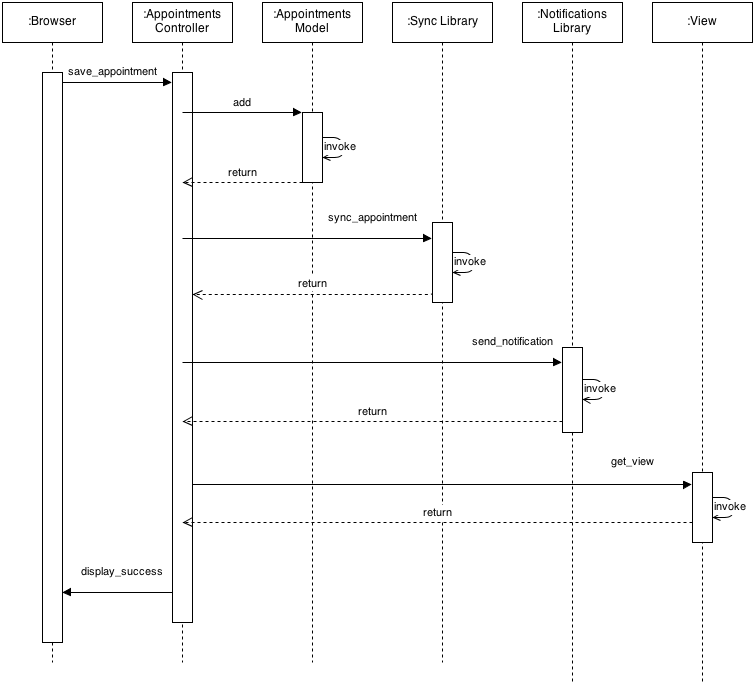
\includegraphics[width=150mm]{images/sd-save-appointment.png}
\caption{Στο διάγραμμα ροής εμφανίζεται η διαδικασία που εκτελείται για την αποθήκευση ενός ραντεβού μετά την επιτυχή καταχώρηση του από τον πελάτη.}
\label{sd-save-appointment}
\end{figure}

\begin{figure}[H]
\centering
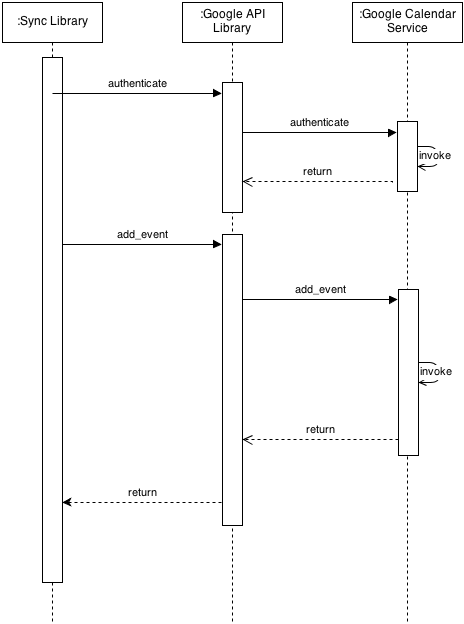
\includegraphics[width=150mm]{images/sd-sync-appointment.png}
\caption{Στο διάγραμμα ροής εμφανίζεται η διαδικασία με την οποία πραγματοποιείται η προσθήκη ενός ραντεβού στο Google Calendar.}
\label{sd-save-appointment}
\end{figure}

\subsection{Διαγράμματα Δραστηριότητας}
Τα διαγράμματα δραστηριότητας αποτελούν γραφικές παραστάσεις της δραστηριότητας του συστήματος ανάλογα με τις αποφάσεις που λαμβάνονται μέσα από τον κώδικα. Σε αυτά τα διαγράμματα μπορούν να φανούν τα σημεία στα οποία υπάρχουν βρόγχοι επανάληψης, τα σημεία όπου μπορούν να συμβούν λογικά σφάλματα (οι απαιτήσεις για συνέχιση της εκτέλεσης δεν πληρούνται) όπως και επίσης τις διαδικασίες που τρέχουν ταυτόχρονα και το πότε γίνεται αυτό.

\begin{figure}[H]
\centering
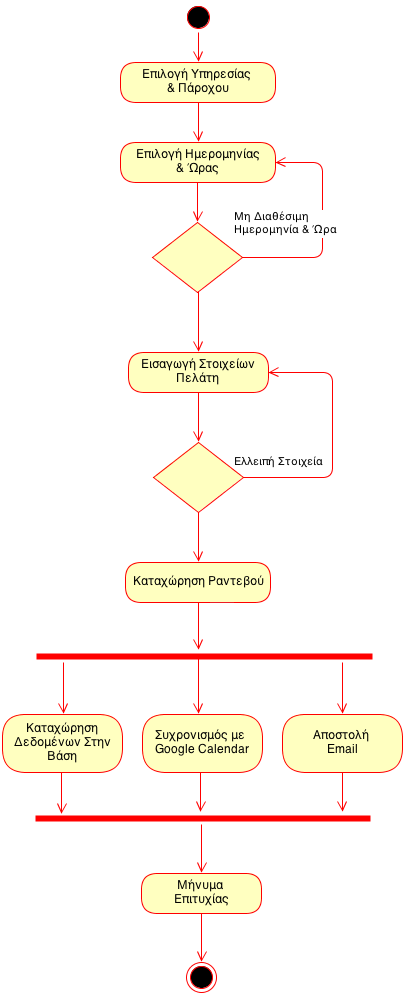
\includegraphics[width=100mm]{images/ad-book-appointment.png}
\caption{Αναπαράσταση της διαδικασίας κράτησης ραντεβού.}
\label{ad-book-appointment}
\end{figure}

\begin{figure}[H]
\centering
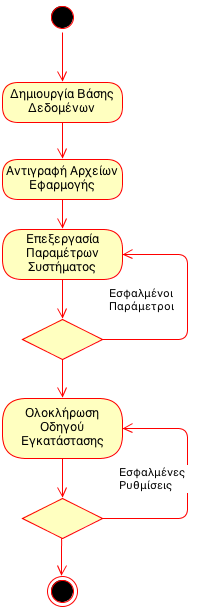
\includegraphics[width=100mm]{images/ad-install-application.png}
\caption{Αναπαράσταση της διαδικασίας εγκατάστασης της εφαρμογής.}
\label{ad-install-application}
\end{figure}

\subsection{Διαγράμματα Κλάσεων}
Στην τεχνολογία λογισμικού, τα διαγράμματα κλάσεων περιγράφουν την στατική δομή ενός συστήματος δείχνοντας τις κλάσεις, τις ιδιότητες, τις λειτουργίες και τις σχέσεις μεταξύ των αντικειμένων. Το σχεδιαγράμματα αυτά είναι τα βασικότερα για έναν προγραμματιστή διότι μπορεί άμεσα να πληροφορηθεί σχετικά με την δομή του κώδικα και με ποιόν τρόπο θα πρέπει να συνεχιστεί η διαδικασία της υλοποίησης.

\begin{figure}[H]
\centering
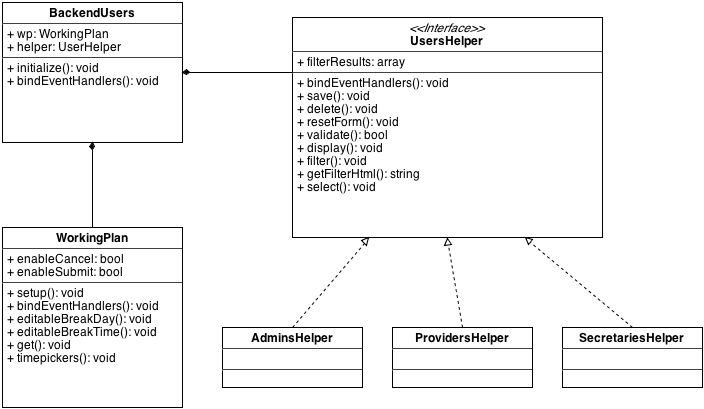
\includegraphics[width=150mm]{images/cd-backend-users.png}
\caption{Στο διάγραμμα αυτό φαίνεται η τρόπος με τον οποίον υλοποιείται η λειτουργικότητα της σελίδας διαχείρισης των χρηστών του συστήματος μέσω της JavaScript. Η κάθε ενότητα διαχείρισης (διαχειριστές, πάροχοι και γραμματείς) έχουν την δικιά τους κλάση, η οποία καθορίζει με ποιόν τρόπο θα χρειαστεί να ανταποκριθεί η εφαρμογή.}
\label{cd-backend-users}
\end{figure}

\begin{figure}[H]
\centering
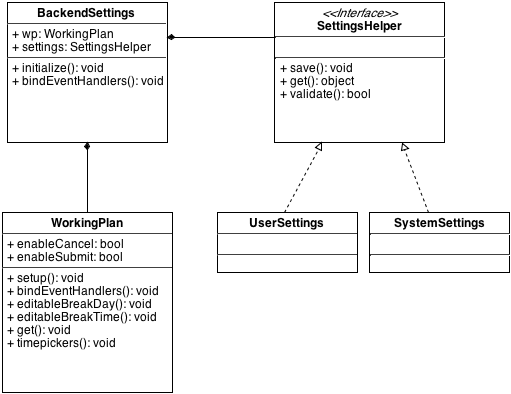
\includegraphics[width=150mm]{images/cd-backend-settings.png}
\caption{Σε αυτό το διάγραμμα κλάσεων φαίνεται οι κλάσεις που συμμετέχουν στον JavaScript κώδικα των κεντρικών ρυθμίσεων της εφαρμογής. Οι κάθε μια κλάση αντιπροσωπεύει την λειτουργία μιας κατηγορίας ρυθμίσεων και μαζί χρησιμοποιούνται για την σωστή λειτουργία της σελίδας.}
\label{cd-backend-settings}
\end{figure}
